\chapter{Eigenvalue analysis of an elastic beam}

\modinfo{Directory}{\Idx{ElasticEigenValues}}
\modinfo{Solvers}{\Idx{StressSolve}, \Idx{EigenSolve}}
\modinfo{Tools}{\Idx{ElmerGrid},Editor}
\modinfo{Dimensions}{3D, Steady-state}

\subsection*{Case definition}

A homogenous, elastic silicon beam of dimensions 1 m length, 0.1 m height and 0.2 m width
is supported on its both ends (boundaries 1 and 2). 
A beam has the density 2330 kg/m$^{3}$, Poisson ratio 0.3 and Young's modulus 10$^{11}$ N/m$^{2}$. The problem is to calculate the eigenvalues of the beam. Mathematically the equation to be solved is
\begin{displaymath}
-\rho \omega^{2}\phi = \nabla\cdot\tau(\phi)
\end{displaymath}
where $\rho$ is the density, $\omega$$^{2}$ is the eigenvalue, $\omega$ is the angular frequency, $\phi$ is the corresponding vibration mode and $\tau$ is the stress tensor.

\begin{figure}[h]
\centering
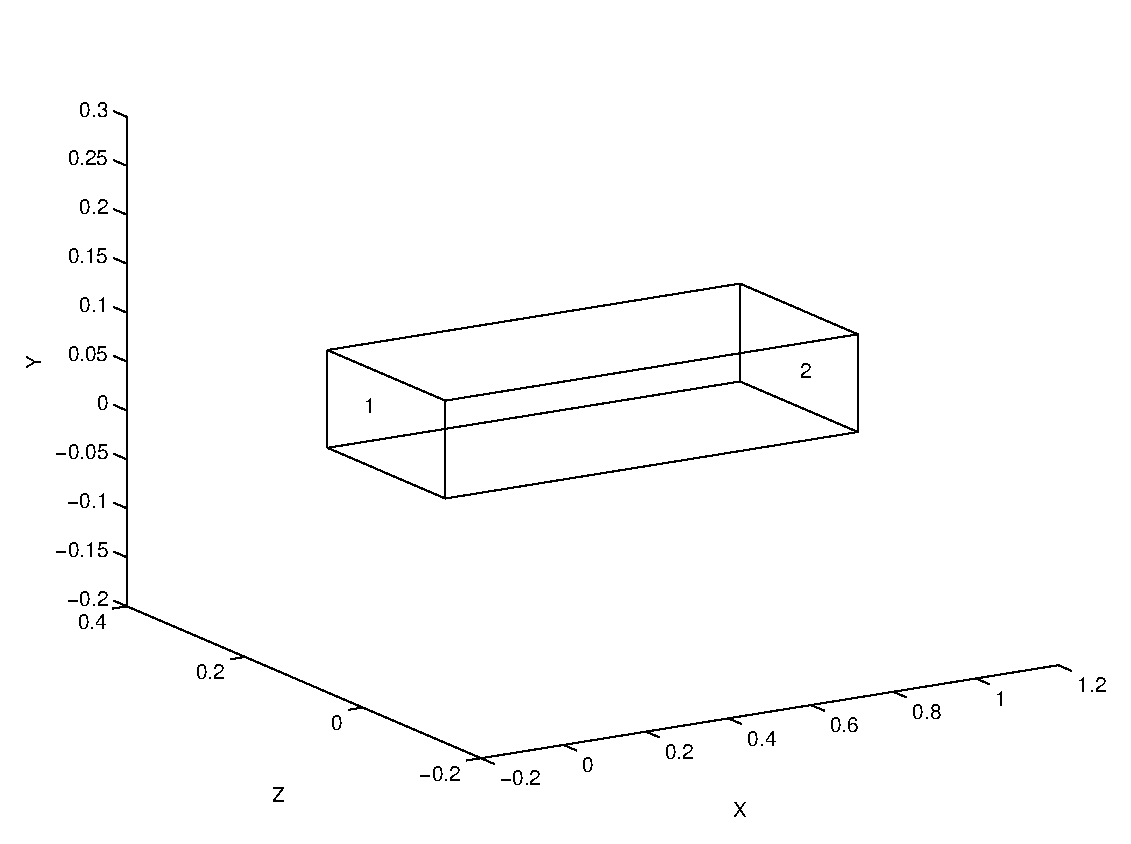
\includegraphics[height=80mm]{palkki}
\caption{Beam.}\label{fg:palkki}
\end{figure}




\subsection*{Solution procedure}

The mesh has been created by using Gambit software and it consists of 2500 elements. The mesh can be converted to Elmer format with ElmerGrid with the command

\ttbegin
ElmerGrid 7 2 mesh.FDNEUT
\ttend

\begin{flushleft}
This command creates the directory which contains the Elmer mesh files.


\ttbegin
Header
  Mesh DB "." "mesh"
  Include Path ""
  Results Directory ""
End
\ttend

A steady-state three-dimensional analysis is defined in the simulation section.

\ttbegin
Simulation
  Coordinate System = "Cartesian 3D"
  Coordinate Mapping(3) = 1 2 3
  Simulation Type = "Steady State"
  Steady State Max Iterations = 1
  Solver Input File = "eigen_values.sif"
  Output File = "eigen_values.dat"
  Post File = "eigen_values.ep"
End
\ttend 

The geometry of the problem is simple and it includes only one body and material. 

\ttbegin
Body 1
  Equation = 1
  Material = 1
End

Material 1
  Youngs Modulus = 100e9
  Poisson Ratio = 0.3
  Density = 2330
End
\ttend

The problem is solved according to linear elastic theory and due to that stress analysis is set to true.

\ttbegin
Equation 1
  Stress Analysis = True
End
\ttend

In the solver section {\tt Stress Analysis} is selected. In addition, the value of the keyword 
{\tt Eigen Analysis} have to set to true. The keyword {\tt Eigen System Values} defines the number of the computed eigenvalues. The problem also is possible to solve with iterative solver but we have used direct solver in this time.

\ttbegin
Solver 1
  Equation = "Stress Analysis"
  Eigen Analysis = Logical True
  Eigen System Values = Integer 5
  Linear System Solver = "direct"

  Variable = "Displacement"
  Variable Dofs = 3
  Linear System Iterative Method = "BiCGStab"
  Linear System Max Iterations = 1000
  Linear System Convergence Tolerance = 1.0e-08
  Linear System Abort Not Converged = True
  Linear System Preconditioning = "ILU0"
  Linear System Residual Output = 1
  Steady State Convergence Tolerance = 1.0e-05
  Nonlinear System Convergence Tolerance = 1.0e-05
  Nonlinear System Max Iterations = 1
  Nonlinear System Newton After Iterations = 3
  Nonlinear System Newton After Tolerance = 1.0e-02
  Nonlinear System Relaxation Factor = 1
  Linear System Precondition Recompute = 1
End
\ttend

The beam is supported on its both ends and therefore displacements is set to zero in all the directions.

\ttbegin  
Boundary Condition 1
  Target Boundaries(1) = 1
  Displacement 1 = 0
  Displacement 2 = 0
  Displacement 3 = 0  
End

Boundary Condition 2
  Target Boundaries(1) = 2
  Displacement 1 = 0
  Displacement 2 = 0
  Displacement 3 = 0  
End
\ttend  

After that, the problem is ready to solve.
\linebreak[4]

\begin{bf}
An anisotropic model
\end{bf}
\linebreak[2]

The same problem can also be solved as an anisotropic problem
which causes a couple of changes in the sif-file.
First, it is reasonable to rename the files in the simulation section

\ttbegin
Solver Input File = "eigen_values_aniso.sif"
Output File = "eigen_values_aniso.dat"
Post File = "eigen_values_aniso.ep"
\ttend

For anisotropic material Young's modulus have to redefine as a matrix. 
In this case the matrix is defined as follows

\ttbegin
Youngs Modulus
Size 6 6
    Real  200e9  60e9   60e9   0     0     0      
          60e9   200e9  200e9  0     0     0      
          60e9   60e9   200e9  0     0     0      
          0      0      0      80e9  0     0      
          0      0      0      0     80e9  0      
          0      0      0      0     0     80e9   
    End
\ttend

No more changes are needed in the sif-file.

\end{flushleft}
\subsection*{Results}
Both the eigenvalues of the isotropic and the eigenvalues of the anisotropic model are shown below in Elmer outputs. Figure \ref{fig:eig12345} presents the computed eigenvectors of the beam with the isotropic model. The formula $\omega$ = 2$\pi$$f$ have been used in calculating frequencies ($f$)
(Table \ref{tb:freq}).
According to the results the anisotropic model yielded greater eigenvalues with
these values of Young's modulus.  


\ttbegin
EigenSolve: Computed Eigen Values:
EigenSolve: --------------------------------
EigenSolve:            1        (16737546.4275755,0.00000000000000D+000)
EigenSolve:            2        (48175589.4544061,0.00000000000000D+000)
EigenSolve:            3        (99674749.0526558,0.00000000000000D+000)
EigenSolve:            4        (110392974.959463,0.00000000000000D+000)
EigenSolve:            5        (253947166.278411,0.00000000000000D+000)

\ttend
\begin{center}
Isotropic model.
\end{center}
\ttbegin
EigenSolve: Computed Eigen Values:
EigenSolve: --------------------------------
EigenSolve:            1        (29608629.8775828,0.00000000000000D+000)
EigenSolve:            2        (88782964.0905879,0.00000000000000D+000)
EigenSolve:            3        (198583949.415515,0.00000000000000D+000)
EigenSolve:            4        (205085884.544046,0.00000000000000D+000)
EigenSolve:            5        (480903841.387323,0.00000000000000D+000)
\ttend
\begin{center}
Anisotropic model.
\end{center}
\begin{table}[h]
\caption{Computed frequencies.}
\label{tb:freq}
\begin{center}
\begin{tabular}{lll} \hline
step  & isotropic & anisotropic\\ \hline
1 & 651.127 Hz  & 866.023 Hz\\
2 & 1104.673 Hz & 1499.633 Hz\\
3 & 1588.959 Hz & 2242.809 Hz\\
4 & 1672.210 Hz & 2279.229 Hz      \\
5 & 2536.249 Hz & 3490.191 Hz    \\ \hline
\end{tabular}
\end{center}
\end{table}


\begin{figure}[h!]
\begin{center}
  \includegraphics[width=0.4\textwidth,angle=0]{eig1}
  \includegraphics[width=0.4\textwidth,angle=0]{eig2}
  \includegraphics[width=0.4\textwidth,angle=0]{eig3}
  \includegraphics[width=0.4\textwidth,angle=0]{eig4}
  \includegraphics[width=0.4\textwidth,angle=0]{eig5}
  \caption{Eigenvectors}
  \label{fig:eig12345}
\end{center}
\end{figure}

\vfill